\chapter{Bento: A toolkit for subcellular analysis of spatial transcriptomics data}
\label{chap:chapter 1}

%%%%%%%%%%%%%%%%%%%%%%%%%%%%%%%%%%%%%%%%%%%%%%%%%%%%%%%%%%%%%%%%%%%%%%%%%%%%%%%%
\section{Introduction}
%%%%%%%%%%%%%%%%%%%%%%%%%%%%%%%%%%%%%%%%%%%%%%%%%%%%%%%%%%%%%%%%%%%%%%%%%%%%%%%%

The spatial organization of molecules in a cell is essential for performing their functions. While protein localization\cite{thulSubcellularMapHuman2017} and disease-associated mislocalization are well appreciated\cite{laurilaPredictionDiseaserelatedMutations2009,parkProteinLocalizationPrincipal2011}, the same principles for RNA have begun to emerge. For instance, the spatial and temporal regulation of RNA play a crucial role in localized cellular processes such as cell migration and cell division\cite{lecuyerGlobalAnalysisMRNA2007,bovairdBiologicalFunctionsRegulatory2018}, as well as specialized cell functionalities like synaptic plasticity\cite{dasTravelsMRNAsNeurons2019,sahooAxonalMRNATransport2018,kugelgenConservationCoreNeurite2020}. Mislocalization of RNA has been associated with diseases such as Huntington's disease (HD), where defects in axonal mRNA transport and subsequent translation in human spiny neurons lead to cell death and neurodegeneration\cite{culverHuntingtonDiseaseProtein2016,romoFreshLookHuntingtin2018,whiteHuntingtinDifferentiallyRegulates2015,fernandopulleRNATransportLocal2021}.

The study of subcellular RNA localization necessitates single-molecule measurements. Since the development of single-molecule fluorescent in situ hybridization (smFISH), recent advances in multiplexed methods such as MERFISH\cite{chenRNAImagingSpatially2015}, seqFISH+\cite{engTranscriptomescaleSuperresolvedImaging2019}, HybISS\cite{gyllborgHybridizationbasedSituSequencing2020}, and Ex-Seq\cite{alonExpansionSequencingSpatially} have enabled RNA localization measurements at near transcriptome scales, while maintaining single-molecule resolution. A number of computational toolkits, such as Squidpy\cite{pallaSquidpyScalableFramework2021}, stLearn\cite{phamStLearnIntegratingSpatial2020}, Giotto\cite{driesGiottoToolboxIntegrative2021}, Seurat\cite{butlerIntegratedAnalysisSingle2017}, and Scanpy\cite{wolfSCANPYLargescaleSinglecell2018} enabled the characterization of tissue architecture, cell-cell interactions, and spatial expression patterns. Despite the single-molecule measurements in spatial transcriptomics, these analytical approaches are limited to investigating spatial variation at the multicellular scale and lack the ability to investigate subcellular organization. To further our understanding of RNA localization and its function in normal and abnormal cell activity, we need to expand our analytical capacity to the subcellular scale.

Recent methods such as FISH-quant-v2\cite{imbertFISHquantV2Scalable2022} and FISHFactor\cite{walterFISHFactorProbabilisticFactor} identify subcellular patterns describing the spatial distribution of RNA species, but are unable to annotate more than a single gene per cell or are limited to analyze at most 20,000 molecules on accessible computing resources. In contrast, a single spatial transcriptomics experiment measures at least hundreds to thousands of genes across hundreds of thousands of cells. Additionally, methods such as ClusterMap\cite{heClusterMapMultiscaleClustering2021} and Baysor\cite{petukhovBayesianSegmentationSpatially2020} highlight the potential for transcript locations alone to inform meaningful domains such as cell and nuclear regions Using spatial proteomics data, CAMPA\cite{spitzerLearningConsistentSubcellular} and Pixie\cite{liuRobustPhenotypingHighly2023} utilize subcellular spatial variation in protein abundance to identify subcellular regions and annotate pixel-level features. 

Building on these promising approaches, we present Bento, an open-source Python toolkit for scalable analysis of spatial transcriptomics data at the subcellular resolution. Bento ingests single-molecule resolution data and segmentation masks, utilizing geospatial tools (GeoPandas\cite{GeopandasGeopandasV0}, Rasterio\cite{gilliesRasterioGeospatialRaster}) for spatial analysis of molecular imaging data, and data science tools including SciPy\cite{virtanenSciPyFundamentalAlgorithms2020}, and Tensorly\cite{kossaifiTensorLyTensorLearning2019} for scalable analysis of high-dimensional feature matrices. Furthermore, Bento is a member of the Scverse ecosystem, enabling integration with Scanpy\cite{wolfSCANPYLargescaleSinglecell2018}, Squidpy\cite{pallaSquidpyScalableFramework2021}, and more than thirty other single-cell omics analysis tools.

%%%%%%%%%%%%%%%%%%%%%%%%%%%%%%%%%%%%%%%%%%%%%%%%%%%%%%%%%%%%%%%%%%%%%%%%%%%%%%%%
\section{Results}
%%%%%%%%%%%%%%%%%%%%%%%%%%%%%%%%%%%%%%%%%%%%%%%%%%%%%%%%%%%%%%%%%%%%%%%%%%%%%%%%

\subsection{Overview of Bento data infrastructure for subcellular analysis}

In order to facilitate a flexible workflow, Bento is generally compatible with molecule-level resolution spatial transcriptomics data (Fig. 1A), such as datasets produced by MERFISH\cite{chenSpatiallyResolvedHighly2015}, seqFISH+\cite{engTranscriptomescaleSuperresolvedImaging2019}, CosMx (NanoString)\cite{heHighplexMultiomicAnalysis2021}, Xenium (10x Genomics)\cite{janesickHighResolutionMapping2022,leeFluorescentSituSequencing2015}, and Molecular Cartography (Resolve Biosciences)\cite{huDynamicControlMetabolic}. Bento's workflow takes as input 1. 2D spatial coordinates of transcripts annotated by gene, and 2. segmentation boundaries (e.g. cell membrane, nuclear membrane, and any other regions of interest) (Fig. 1B). While 3D molecular coordinates are commonly included, 3D segmentation information is limited to z-stacked 2D segmentation, limiting its usability. If available, Bento can also handle arbitrary sets of segmentations for other subcellular structures or regions of interest. These inputs are stored in the AnnData data format\cite{virshupAnndataAnnotatedData2021}, which links cell and gene metadata to standard count matrices, providing compatibility with standard single-cell RNA-seq quality control and analysis tools in the Scverse ecosystem\cite{wolfSCANPYLargescaleSinglecell2018}. With a data structure for segmentation boundaries and transcript coordinates in place, Bento can easily compute spatial statistics and measure spatial phenotypes to build flexible multidimensional feature sets for exploratory subcellular analysis and utilize these spatial metrics to augment quality control (Fig. 1C).

\begin{figure}[h]
    \centering
    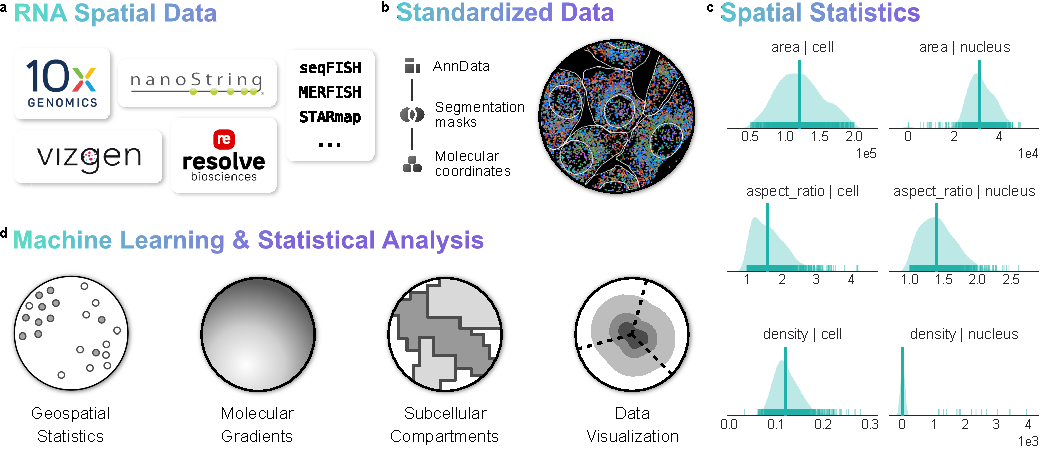
\includegraphics[width=\textwidth]{1_figures-and-files/Fig1.pdf}
    \caption[Workflow and functionality of the Bento toolkit.]{\textbf{Workflow and functionality of the Bento toolkit.} A. Single-molecule resolved spatial transcriptomics data from commercial or custom platforms are ingested into Bento where it is converted to the AnnData format (B.), where it can be manipulated with Bento as well as a wide ecosystem of single-cell omics tools. C. Geometric statistics are illustrated for the seqFISH+ dataset, including metrics describing cell and nuclear geometries and cell density to assess overall data quality. D. Bento has a standard interface to perform a wide variety of subcellular analyses.}
    \label{fig:1 bento overview}
\end{figure}

Bento offers a precise yet flexible palette of novel complementary subcellular analyses (Fig. 1D). We present RNAforest, a multilabel approach for annotating RNA localization patterns adapted from FISH-quant v2\cite{imbertFISHquantV2Scalable}. We find that many RNAs are spatially distributed according to gene function. We then implement RNAcoloc, a context-specific approach to quantify colocalization to characterize how genes colocalize with each other in a compartment-specific manner. Having established systematic patterning and organization of RNA transcripts, we demonstrate RNAflux, an unsupervised method for semantic segmentation of subcellular domains. RNAflux first quantifies subcellular expression gradients at pixel resolution before identifying consistent subcellular domains via unsupervised clustering. We demonstrate the utility of Bento's tools characterizing subcellular organization in two spatial transcriptomics datasets, a 10k gene MERFISH dataset of U2-OS cells and a 130 gene seqFISH+ dataset of 3T3 cells. We find that RNA localization patterns are associated with known gene function, and that genes with similar localization patterns are functionally related. We also find that genes with similar localization patterns are co-regulated at the transcriptional level. Finally, we find that RNAflux identifies subcellular domains that are consistent across cells and are associated with known subcellular structures.



\subsection{RNAforest: Utilizing subcellular landmarks to predict RNA subcellular localization}

In computer vision, key points or landmarks are commonly used for tasks like facial recognition\cite{violaRapidObjectDetection2001} and object detection. Analogous to these classical applications, we derive spatial features using cell and nucleus boundaries as landmarks to predict RNA localization patterns from spatial summary statistics. Building on the summary statistics used for classifying smFISH data in FISH-quant v2\cite{imbertFISHquantV2Scalable2022}, RNAforest consists of an ensemble of five binary random forest classifiers rather than a single multi-classifier model to assign one or more labels. These pattern labels, adapted from several high-throughput smFISH imaging experiments in HeLa cells\cite{battichImagebasedTranscriptomicsThousands2013,stoegerComputerVisionImagebased2015,samacoitsComputationalFrameworkStudy2018,chouaibDualProteinmRNALocalization2020}, are broadly applicable to eukaryotic cells: (i) nuclear (contained in the volume of the nucleus), (ii) cytoplasmic (diffuse throughout the cytoplasm), (iii) nuclear edge (near the inner/outer nuclear membrane), (iv) cell edge (near the cell membrane), and (v) none (complete spatial randomness). It is important to note, as was done previously in  FISH-quant v2\cite{imbertFISHquantV2Scalable2022} that because of the 2D nature of the dataset, RNA that is in truth cytoplasmic but above or below the nucleus will still appear as though in the nucleus when collapsed in the z-dimension. As we use the FISH-quant v2 pattern simulation framework, this is accounted for in the training dataset.

We used the FISH-quant v2 simulation framework to generate realistic ground-truth data\cite{samacoitsComputationalFrameworkStudy2018}. Each sample is defined as a set of points with coordinates in two dimensions, representing the set of observed transcripts for a gene in a particular cell. In total, we simulated 2,000 samples per class for a total of 10,000 samples (Methods). We used 80\% of the simulated data for training and held out the remaining 20\% for testing. Each sample is encoded by a set of 13 input features, describing characteristics of its spatial point distribution, including proximity to cellular compartments and extensions (features 1-3), measures of symmetry about a center of mass (features 4-6), and measures of dispersion and point density (feature 7-13) (Fig. 2A). These features are normalized to morphological properties of the cell to control for variability in cell shape. A detailed description of every feature is described in Supp. Table 1. 

\begin{figure}[p]
    \centering
    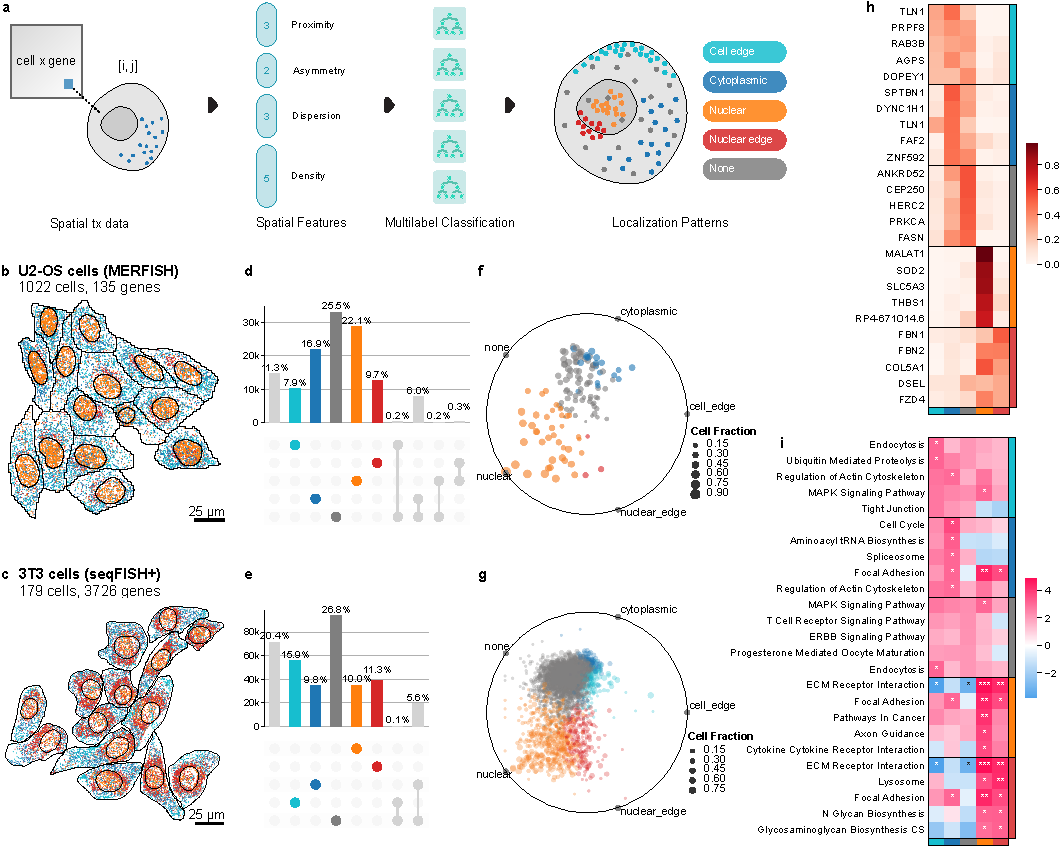
\includegraphics[width=\textwidth]{1_figures-and-files/Fig2.pdf}
    \caption[Subcellular localization pattern identification with RNAforest.]{\textbf{Subcellular localization pattern identification with RNAforest.} A. Thirteen spatial summary statistics are computed for every gene-cell pair describing the spatial arrangement of molecules and boundaries in relation to one another. The features are inputs for RNAforest, a multilabel ensemble classifier which assigns one or more subcellular localization labels: cell edge, cytoplasmic, nuclear, nuclear edge, and none. Top 10 genes for each label visualized for each label other than “none” in B. U2-OS cells, and C. 3T3 cells. D. and E. show the proportion of measured transcripts assigned to each label. F. and G. show the relative label proportion across cells for each gene and is colored by the majority label (F and G). H. Top 5 consistent genes for each label. I. ssGEA identifies enrichment of GO cellular component domains for each label in the 3T3 cell dataset.
    }
    \label{fig:2 RNAforest localization pattern identification}
\end{figure}

We applied RNAforest on the MERFISH dataset measuring 130 genes (low plexity) in U2-OS cells and high detection efficiency per gene (111 molecules per gene per cell on average), and on the seqFISH+ dataset measuring 10,000 genes (very high plexity) but lower detection efficiency (8 molecules per gene per cell on average) (Fig. 2B-C, Supp. Fig. 1). In agreement with previous work characterizing RNA localization of 411 genes\cite{chouaibDualProteinmRNALocalization2020}, we find that genes commonly exhibit variability in localization across cells. This suggests that heterogeneity in localization likely generalizes to the entire transcriptome. Of the localization patterns besides ``none'', ``nuclear'' was the most common (22.1\%) in the U2-OS osteosarcoma cells (Fig. 2D \& 2F), while ``cell edge'' was the most common (15.9\%) in the 3T3 fibroblast cells (Fig. 2E \& 2G). 

In the U2-OS cells, we found many genes to have preferential localization in different subcellular compartments (Fig. 2H). In agreement with our RNAflux findings, we find genes known to localize to the nucleus\cite{moffittHighthroughputSinglecellGeneexpression2016,kumarIntracellularSpatialTranscriptomic2023} to be frequently labeled ``nucleus'' (MALAT1, SOD2) and genes encoding secreted extracellular proteins\cite{chenRNAImagingSpatially2015} to be frequently labeled ``nuclear edge'' (FBN1, FBN2). As expected, we find genes preferentially ``nuclear'' and ``nuclear edge'' localized to mirror nucleus and endoplasmic reticulum genes found in a 10k genes MERFISH study of U2-OS cells that included ER staining\cite{xiaSpatialTranscriptomeProfiling2019} (Supp. Fig. 2, Methods). Leveraging the 3T3 seqFISH+ dataset's higher plexity, we were able to ask whether genes with similar localization preference are functionally related. We applied gene set enrichment analysis to gene localization frequencies to identify enriched gene ontology terms\cite{thegeneontologyconsortiumGeneOntologyResource2021} (Fig. 2I, Methods). Secretory processes were enriched in the nucleus and nuclear edge, which may be linked to increased transcription of fibroblast-related functions. Cell edge enriched pathways consisted of those with the cell membrane as their site of function (e.g. endocytosis and tight junction suggesting local translation of these genes). Additionally, the term for cell cycle was significantly enriched in the cytoplasm only. Genes without strong localization preference (most frequently ``none'') were not significantly associated with any pathways. These genes likely do not undergo active transport and are functionally independent of local translation. 
RNAforest gives a user a facile method for annotating RNA localization patterns and quantifying heterogeneity in a transcriptome-wide manner independent of RNA abundance. Beyond known RNA localizations, we find that transcript location is generally associated with known gene function, alluding to the systematic spatial regulation of RNA transport. We foresee RNAforest will be a valuable addition to characterize RNA localization across diverse spatial transcriptomics datasets. 

\subsection{RNAcoloc: An approach for context-specific RNA colocalization}

In geospatial information processing, a fundamental feature that is often gleaned from large datasets is the colocation of objects (e.g. gleaning socialization metrics from cell phone colocation data in Singapore\cite{xuHowFriendsShare2017}). Colocation is similarly valuable in understanding co-translation and interaction networks of genes in a biological context\cite{zengSpatiallyResolvedSinglecell2023}. Recent spatial transcriptomics approaches have used a number of colocalization metrics from the geographic information systems and ecology fields e.g. the bivariate versions of the Ripley's K function (also known as cross-k-function)\cite{ripleySecondorderAnalysisStationary1976}, Moran's I\cite{tiefelsdorfModellingSpatialProcesses2006}, and the join count statistic\cite{cliffSpatialProcessesModels1981}. These metrics are designed to measure spatial associations between two populations i.e. gene A transcripts and gene B transcripts. However, it is more appropriate to think of all transcripts in a single cell from a single population; after all, RNA transcription and localization is not completely stochastic. We have shown that the subcellular distribution of RNA is highly structured with RNAforest. As such, we developed RNAcoloc, an approach that combines  the Colocation Quotient (CLQ)\cite{leslieColocationQuotientNew2011} metric and tensor decomposition for context-specific RNA colocalization (Methods). The CLQ is a colocalization statistic that is capable of accounting for the biophysical properties of RNA spatial distributions. First, the CLQ considers how clustered the overall RNA population is in a cell and measures whether specific pairs of genes are more clustered than expected given the spatial pattern of the overall population. Second, the CLQ is inherently asymmetric, and captures the direction of attraction i.e. the attraction of gene A to gene B is not the same as the attraction of gene B to gene A. This is most common when gene A and gene B have very different expression levels, which is prevalent due to overdispersion in gene expression data.

RNAcoloc calculates CLQ scores for each gene per cell in a compartment-specific manner, such that each sample has 2 scores, a nucleus and cytoplasm CLQ score. An initial comparison of global colocalization between nuclear and cytoplasmic fractions unsurprisingly found that transcripts from the same gene tend to cluster more tightly with themselves than with transcripts from other genes (Fig. 3B). Additionally, self-colocalization is significantly stronger in the cytoplasm than in the nucleus. In conjunction with our findings from RNAforest analysis that genes of the same localization pattern tend to have similar functions, this suggests that the RNAs are more tightly spatially regulated once exported from the nucleus. 

By calculating CLQ scores for every gene-gene pair across compartments, RNAcoloc constructs a tensor of shape P x C x S where P, C, and S represent the number of gene-gene pairs, cells, and compartments, respectively (Fig. 3A, Methods). 

RNAcoloc then applies tensor decomposition — specifically, non-negative parallel factor analysis — a data-driven, unsupervised approach for discovering substructure in high-dimensional data\cite{kossaifiTensorLyTensorLearning2019,shashuaNonnegativeTensorFactorization2005} to decompose the U2-OS dataset colocalization tensor into k = 4 ``colocalization factors''. The number of factors was determined using the elbow method heuristic, optimizing for the root mean squared error (RMSE) reconstruction loss (Methods). Unlike matrix dimensionality reduction methods, such as PCA, the order of the components (factors) is unassociated with the amount of variance explained. Each of the 4 colocalization factors is composed of 3 loading vectors, which correspond to the compartments, cells and gene pairs. Higher values denote a stronger association with that factor. Crucially for interpretation, factors derived from tensor decomposition are not mutually exclusive and share overlapping sets of associated compartments, cells, and gene pairs.

\begin{figure}[p]
    \centering
    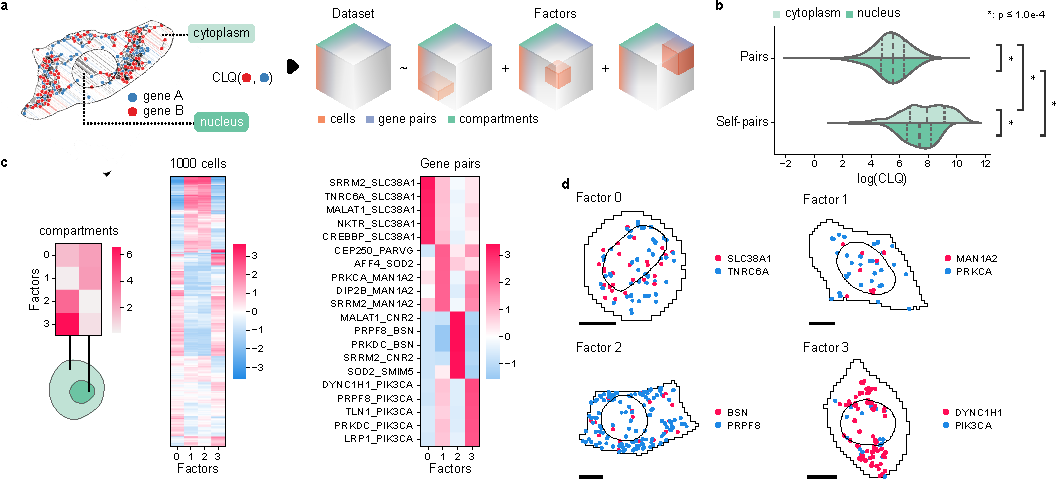
\includegraphics[width=\textwidth]{1_figures-and-files/Fig3.pdf}
    \caption[Compartment-specific RNA colocalization with RNAcoloc.]{\textbf{Compartment-specific RNA colocalization with RNAcoloc.} A. Transcripts are separated by compartment (nucleus and cytoplasm) before CLQ scores are calculated for every gene pair across all cells. This yields a cell x gene pair x compartment tensor. B. Comparison of log CLQ distributions for gene pairs and self-pairs, further categorized by compartment. C. Tensor decomposition yields 4 factors. From left to right, the three heatmaps show the loadings of each factor for each dimension – compartments, cells, and gene pairs. Only the top 5 associated gene pairs for each factor are shown. D. Top examples of compartment-specific colocalized gene pairs. Black scale bars denote 10 um.
    }
    \label{fig:3 RNAcoloc colocalization analysis}
\end{figure}

These trends are broken down into unique combinations of colocalization behavior (Fig. 3C). Factor 0 captures gene pairs in a subpopulation of cells that tend to colocalize across the entire cell, with pairs including SLC38A1 showing the strongest signal. Factor 3 describes gene pairs in mostly the same cell subpopulation, that colocalize specifically in the cytoplasm. Pairs including PIK3CA dominate this behavior. Interestingly, PIK3CA and DYNC1H1 transcripts colocalize cytoplasmically. While little is known about their RNA interactions, PIK3CA and other members of the PI3K pathway are known regulators of mitotic organization, including the regulation of dynein and dynactin motor proteins. DYNC1H1 specifically encodes cytoplasmic dynein, a motor protein critical for spindle formation and chromosomal segregation in mitosis\cite{gassmannDyneinKinetochore2023}. In the complementary cell population, Factors 1 and 2 highlight colocalized gene pairs in the nucleus and cytoplasm respectively. Notably, Factor 2 associated cells have high loadings for MALAT1 and CNR2 in the cytoplasm and low loadings in the nucleus. Even though MALAT1 is abundantly localized to the nucleus, this demonstrates that the CLQ score identifies gene pairs colocalizing more than expected given the overabundance of MALAT1 relative to CNR2, whereas other approaches seem confounded by large differences in expression\cite{kumarIntracellularSpatialTranscriptomic2023}.

We demonstrate the ability of RNAcoloc to quantify compartment-specific gene-pair colocation by exploring cytoplasmic vs. nuclear colocalization. As we found separately with RNAforest, RNAcoloc analysis finds evidence that RNA transport is spatially regulated, especially after nuclear export. We highlight several examples of colocalization suggesting how RNA localization allows the same gene to have multiple functions in a spatially-dependent fashion i.e. depending on its molecular neighbors and local environment\cite{guptaMoonlightingEnzymesWhen2023,gnannIlluminatingNongeneticCellular2021}. We foresee RNAcoloc will be increasingly relevant as many spatial technologies are beginning to image proteins along with RNA, which can be used to delineate more granular  compartments, such as cell organelles or distinct regions e.g. neuron cell bodies vs dendrites. 

\subsection{RNAflux: Unsupervised semantic segmentation of subcellular domains in single cells}

To build on RNAforest, we overcame the restricted number of localization patterns defined by the supervised method by framing RNA localization as an unsupervised embedding problem. RNAflux looks at local neighborhoods within the space of a cell and builds a normalized gene composition per neighborhood. Differences in neighborhood compositions can be leveraged to identify distinct subcellular domains in a manner that is entirely unsupervised and independent of cell geometry.

We applied this embedding procedure to compute a gene composition vector for every pixel in 2D coordinate space, generating a spatial composition gradient across entire cells (Fig. 4A, Methods). 

Applied to a MERFISH dataset with a target panel of 130 genes across over 1153 U2-OS cells, we demonstrate that RNAflux embeddings can detect transcriptionally distinct subcellular domains. Performing dimensional reduction of the embeddings showed that the top sources of variation spatially correspond to the nucleus, the nuclear periphery, and cytoplasmic regions consistently across cells (Fig. 4B, Methods) confirming that RNAflux measures intracellular transcriptional variation, as opposed to intercellular variation. To delineate compositionally similar domains in a data-driven manner, we cluster pixel embeddings using self-organizing maps (SOMs), effectively performing unsupervised semantic segmentation (Methods). We denote the resulting clusters as “fluxmap domains”. We found that this assigned pixels to 5 fluxmap domains, consistently highlighting spatial regions across every cell (e.g. fluxmap 2 is always nuclear while the remaining domains constitute the cytoplasm) (Fig. 4B). By considering the spatial distribution of molecules across fluxmap domains, we can quantify the composition of molecules for each gene across fluxmaps (Fig. 4C) e.g. nuclear-localized MALAT1 \cite{moffittHighthroughputSinglecellGeneexpression2016,kumarIntracellularSpatialTranscriptomic2023}.

\begin{figure}[p]
    \centering
    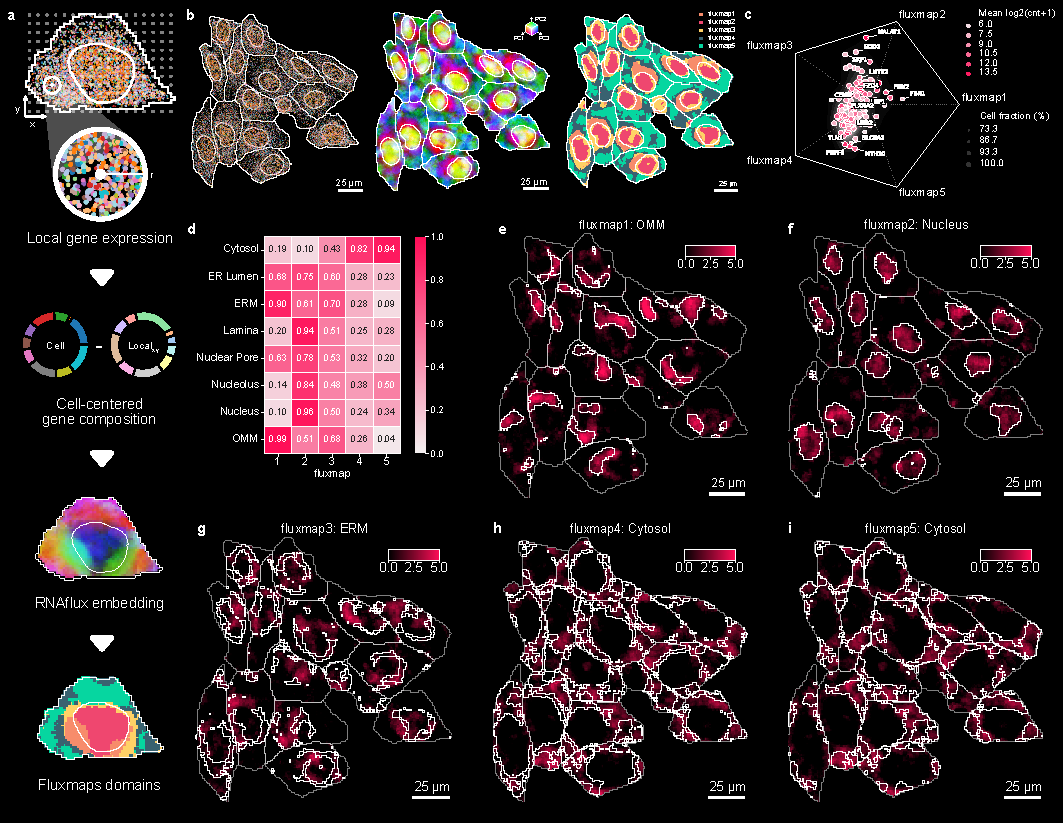
\includegraphics[width=\textwidth]{1_figures-and-files/Fig4.pdf}
    \caption[RNAflux finds distinct subcellular domains with consistent spatial organization and local gene composition.]{\textbf{RNAflux finds distinct subcellular domains with consistent spatial organization and local gene composition.} A. Flowchart of RNAflux and fluxmap computation. Local neighborhoods of a fixed radius are arrayed across a cell and a normalized gene composition is computed for each pixel coordinate, producing an RNAflux embedding. The first three principal components of the RNAflux embedding are visualized for U2-OS cells coloring RGB values by PC1, PC2, and PC3 values respectively for each pixel. Fluxmap domains are computed from each RNAflux embedding to create semantic segmentation masks of each subcellular domain. B. The left panel shows a field of view of U2-OS cells, dots denoting individual molecules colored by gene species, nuclei and cell boundaries outlined in white. For the same field of view of cells, the center panel shows RNAflux embeddings and the right panel shows fluxmap domains. C. The scatter plot shows how the composition of each gene is distributed across fluxmap domains. The position of each point denotes the relative bias of a given gene's composition across fluxmaps. D. Heatmap showing the fraction of pixels with a positive enrichment value for each APEX-seq location for each fluxmap domain.  E-I. The most highly enriched location is shown for each fluxmap domain. Domain boundaries are denoted by white lines within each cell.}
    \label{fig:4 RNAflux finds dinstinct subcellular domains}
\end{figure}

Finally, we sought to characterize the fluxmap domains with known information about RNA localization. We used data from a previous study that measured gene expression at “distinct subcellular locales” via APEX-seq, a technique for proximity labeling and sequencing of RNA\cite{fazalAtlasSubcellularRNA2019}. Of the 3288 genes differentially enriched to one or more locales, 63 overlapped with the 130 MERFISH genes. The location enrichment score for each pixel is calculated by taking the weighted sum of its RNAflux embedding and the measured relative enrichment i.e. log fold change measured by APEX-seq loadings for a given organelle-specific geneset (Methods). Visualizing each pixel's location-specific enrichment scores from the APEX-seq dataset highlights the subcellular localization of these compartments, including the cytosol, nucleus, nucleolus, nuclear pore, nuclear lamina, endoplasmic reticulum lumen (ER lumen), ER membrane (ERM), and the outer mitochondrial membrane (OMM) (Fig. 4D). We find the nuclear compartments have high scores in domain 2, while the cytoplasm scores rank highest in domains 4 and 5. Both the ERM and OMM scores are the strongest in domain 1 (Fig. 4E).

In summary, RNAflux finds distinct subcellular domains with consistent spatial organization and local gene composition. As an unsupervised method, RNAflux can be applied to any cell type for inferring subcellular domains from transcript locations and functionally annotated with biological enrichment analysis.


%%%%%%%%%%%%%%%%%%%%%%%%%%%%%%%%%%%%%%%%%%%%%%%%%%%%%%%%%%%%%%%%%%%%%%%%%%%%%%%%
\section{Discussion}
%%%%%%%%%%%%%%%%%%%%%%%%%%%%%%%%%%%%%%%%%%%%%%%%%%%%%%%%%%%%%%%%%%%%%%%%%%%%%%%%

Bento seeks to interrogate biology via its “subcellular first” approach to spatial analysis, complementary to “cell-type or tissue first” spatial analysis methods. The toolkit enables quantitative, reproducible, and accessible analysis agnostic of spatial technology platforms in a standardized framework. We implement three novel methods to interrogate subcellular RNA organization: RNAforest for supervised annotation of localization patterns, RNAcoloc for compartment-aware colocalization analysis, and RNAflux for identifying transcriptionally distinct subcellular domains. We showed that with RNAflux, we were able to quantify RNA localization in a variety of contexts, including domain-specific gene localization, drug-induced changes in localization, and cell type specific localization. With both RNAflux and RNAforest, we find that subcellular mRNA localization reflects gene function. With RNAcoloc, we explore the use of CLQ scores to quantify pairwise gene colocalization with the context of asymmetric associations. 

From these results, we found three main factors to limit the effectiveness of subcellular-resolution analysis: molecule density, segmentation quality, and target panel composition. In particular, RNAflux becomes uninformative if too few molecules are detected per cell or if the number of molecules per gene is too sparse. We found that datasets with higher density i.e. molecules per micrometer2 are less noisy and inform more coherent gradients and domains, such as the U2-OS dataset. In contrast, RNAforest performs reliably beyond a minimum of 5-10 molecules per sample, but is sensitive to accurate segmentation for calculating cell morphology-dependent features. The 3T3 cells were manually segmented and the U2-OS cells had relatively accurate segmentation, and were therefore amenable to applying RNAforest.  In the case of RNAcoloc, the limiting factor to identify relevant biology is target panel composition. The current focus of most target panels typically include cell type markers and highly expressed genes, whereas it would be more informative to identify colocalizing members of protein complexes, functional pathways, or ligand-receptor pairs. 

A dimensional limitation of Bento is its current inability to process three-dimensional spatial transcriptomic data. While some commercially available spatial transcriptomic methods yield RNA molecular coordinates in 3D, the nuclear and cell segmentation is inevitably still two dimensional making it difficult to interpret z-dimensional positions lacking the context of cellular geometry in 3D. However, the algorithms behind RNAforest, RNAcoloc, RNAflux, and the plethora of feature calculation functions in Bento are inherently extensible to leveraging three dimensionality. When three dimensional cell segmentation improves, we intend to extend Bento to support three dimensional analysis.

\section{Conclusion}

Conventionally, RNA is treated as an intermediary vehicle encoding genomic information for protein synthesis. We began our investigation of RNA localization with the hope of understanding how the spatial organization of RNA functions as a mechanism for post-transcriptional regulation. However, RNAflux conceptually introduces using RNA molecular coordinates as a latent layer of information encoding cellular space-time. Here, we used that latent layer of information to identify subcellular domains. As spatial omic technologies improve to capture more and more information, the potential applications of such latent embeddings will grow as well. Indeed at the tissue level, this concept is already being leveraged with a recent tool, TensionMap, using RNA localization information to predict mechanical tension\cite{hallouComputationalPipelineSpatial2023}. As applications for spatial transcriptomics grow in popularity and complexity, we hope Bento is a platform for the tools needed to quantify the complex molecular dynamics governing normal and abnormal cellular processes.

%%%%%%%%%%%%%%%%%%%%%%%%%%%%%%%%%%%%%%%%%%%%%%%%%%%%%%%%%%%%%%%%%%%%%%%%%%%%%%%%
\section{Methods}
%%%%%%%%%%%%%%%%%%%%%%%%%%%%%%%%%%%%%%%%%%%%%%%%%%%%%%%%%%%%%%%%%%%%%%%%%%%%%%%%

\subsection{MERFISH and seqFISH+ data preprocessing}
For the seqFISH+ dataset, we limited the scope of our analysis to the set of genes for which at least 10 molecules were detected in at least one cell. This helped reduce sparsity in the data, resulting in 3726 genes remaining. Because pattern classification requires nuclear segmentation masks, we removed all cells lacking annotated nuclei for a remainder of 179 cells. Because the MERFISH data had a much higher number of molecules detected per gene, no gene needed to be removed. Again, cells without annotated nuclei were removed, leaving 1022 cells for downstream analysis.

\subsection{RNAforest: model selection and training}
We evaluated 4 base models for the multilabel classifier including random forests (RF), support vector machines (SVM), feed-forward fully-connected neural networks (NN), and convolutional neural networks (CNN). While all other models use the 13 spatial features for input (Supp. Table 1), the CNN takes 64x64 image representations of each sample as input. Each multilabel classifier consists of 5 binary classifiers with the same base model. We used the labeled 10,000 simulated samples for training, stratifying 80\% of the simulated data for training and holding out the remaining 20\% for testing. To select the best hyperparameters for each multilabel classifier, we sampled from a fixed hyperparameter space with the Tree-structured Parzen Estimator algorithm, and evaluated performance with 5-fold cross validation (Supp. Table 3). We retrained the final model (random forest base model) on all training data with the best performing set of hyperparameters (Supp. Fig. 1E).

\subsection{RNAforest: Image rasterization of molecules and segmentation masks for CNN}
To generate an image for a given sample, point coordinates, the cell segmentation mask and nuclear segmentation mask are used. The area of the cell is tiled as a 64 x 64 grid, where each bin corresponds to a pixel in the final image. Values are stored in a single channel to render a grayscale image. Pixels inside the cell are encoded as 20, inside the nucleus encoded as 40. Bins with molecules are encoded as (40 + 20 x n) where n is the number of molecules. Finally values are divided by 255 and capped to be between 0 and 1.

\subsection{RNAforest: Simulating training data}
We trained a multilabel classifier to assign each gene in every cell labels from five categories: (i) nuclear (contained in the volume of the nucleus), (ii) cytoplasmic (diffuse throughout the cytoplasm), (iii) nuclear edge (near the inner/outer nuclear membrane), (iv) cell edge (near the cell membrane), and (v) none (complete spatial randomness). These categories are a consolidation of those observed in several high-throughput smFISH imaging experiments in HeLa cells\cite{battichImagebasedTranscriptomicsThousands2013,stoegerComputerVisionImagebased2015,samacoitsComputationalFrameworkStudy2018,chouaibDualProteinmRNALocalization2020}. We used the FISH-quant simulation framework to generate realistic ground-truth images using empirically derived parameters from the mentioned high-throughput smFISH imaging experiments in HeLa cells \cite{samacoitsComputationalFrameworkStudy2018}. In total, we simulate 2,000 samples per class for a total of 10,000 training samples.

\begin{enumerate}
    \item Cell shape: Cell morphology varies widely across cell types and for classifier generalizability, it is important to include many different morphologies in the training set. We use a catalog of cell shapes for over 300 cells from smFISH images in HeLa cells that captures nucleus and cell membrane shape\cite{samacoitsComputationalFrameworkStudy2018}. Cell shapes were obtained by cell segmentation with CellMask and nuclear segmentation was obtained from DAPI staining.
    \item mRNA abundance: We simulated mRNA abundance at three different expression levels (40, 100, and 200 mRNA per average sized cell) with a Poisson noise term. Consequently, total mRNA abundance per cell was between 5 and 300 transcripts.
    \item Localization pattern: We focused on 5 possible 2D localization patterns, including cell edge, cytoplasmic, none, nuclear, and nuclear edge. Each pattern was further evaluated at 3 different degrees - weak, moderate, and strong. Moderate corresponds to a pattern typically observed in a cell, whereas weak is close to spatially random. These 5 classes aim to capture biologically relevant behavior generalizable to most cell types; there is room for additional classes describing other biologically relevant localization patterns so long as they can be accurately modeled.
    \item RNAforest: Manual annotation of validation data
    \begin{enumerate}
        \item Using 3 individual annotators, we annotated the same 600 samples across both datasets, keeping samples with 2 or more annotator agreements as true annotations, resulting in 165 annotated seqFISH+ samples and 238 annotated MERFISH samples (403 total).
        \item We used Cohen's kappa coefficient\cite{cohenCoefficientAgreementNominal1960} to calculate agreement between pairs of annotators for each label yielding an overall coefficient of 0.602.
        \item We found that pairwise agreement between annotators across labels was fairly consistent ranging between 0.588 and 0.628, while label-specific agreement varied more, ranging between 0.45 and 0.72 (Supp. Table 4).
    \end{enumerate}
\end{enumerate}

\subsection{RNAforest: Functional enrichment of gene pattern distributions}
For enrichment of compartment-specific expression from Xia et al 2019\cite{xiaSpatialTranscriptomeProfiling2019}, scores are calculated by taking the weighted sum of gene pattern frequencies and published compartment log fold-change values (Supp. Fig. 2). The Benjamini-Hochberg correction was used to correct p-values for multiple hypothesis testing. For the seqFISH+ dataset, we performed single-sample Gene Set Enrichment Analysis\cite{subramanianGeneSetEnrichment2005,barbieSystematicRNAInterference2009} on gene pattern frequencies to compute enrichment scores (Fig. 2I). ssGSEA was performed with the GSEApy Python package and the ``GO\_Cellular\_Component\_2021'' gene set library curated by Enrichr\cite{xieGeneSetKnowledge2021}. Gene sets with a minimum size of 50 and a maximum size of 500 were analyzed. 

\subsection{Colocation quotient for RNA colocalization analysis}
Pairwise colocalization of genes was determined for each compartment of every cell separately. In this case, each cell was divided into compartments, cytoplasm and nucleus. The colocation quotient (CLQ) was calculated for every pair of genes \(A\) and \(B\). The CLQ is defined as an odds ratio of the observed to expected proportion of \(B\) transcripts among neighbors of \(A\) for a fixed radius r; it is formulated as:

\[CLQ_{A \rightarrow B} = \frac{C_{A \rightarrow B} / N_A}{N^{A}_{B} / N-1}\]

Here \(C_{A \rightarrow B}\) denotes the number of \(A\) transcripts of which \(B\) transcripts are considered a neighbor. \(N_A\) denotes the total number of A transcripts, while \(N_B\) stands for the total number of B transcripts. In the case that \(A=B\), \(N_B\) equals the total number of B transcripts minus one. \(N\) denotes the total number of transcripts in the cell. Following statistical recommendations from the original formulation of the colocation quotient (CLQ), genes with fewer than 10 transcripts were not considered to reduce sparsity and improve testing power\cite{leslieColocationQuotientNew2011}.

\subsection{Tensor decomposition for compartment-specific colocalization}
For tensor decomposition, we employed non-negative parallel factor analysis as implemented in Tensorly\cite{kossaifiTensorLyTensorLearning2019}, which seeks to represent our dataset tensor \(X\) in a lower dimensional space of \(R\) signatures by decomposing \(X\) as the sum of \(R\) rank-one 3-way tensors. Each of these tensors is described as the outer product of 3 vectors, xr, yr and zr. The collection of vectors across R signatures we denote as \(x^r\) (compartment loadings), \(y^r\) (cell loadings) and \(z^r\) (gene pair loadings) respectively. We find the optimal rank-\(R\) decomposition of \(X\) by minimizing reconstruction error as a function of the number of signatures \(R\) and use the elbow function heuristic to choose the best-fit across the range of 2-12 factors. Missing values are ignored when calculating the loss.

\[X = \sum_{r=1}^{R} x^r y^r z^r\]

\subsection{RNAflux: Unsupervised spatial embedding and subcellular domain quantization}
To generate RNAflux embeddings, first a set of query coordinates are generated tiling across the cell area on a uniform grid. This effectively downsamples the original data units (pixels) resulting in much fewer samples to compute embeddings. For the MERFISH U2-OS dataset, a step size of 10 data units (pixels) was used to generate the uniform grid. Each query point is assigned an expression vector, counting the abundance of each gene within a fixed radius of 40 and 50 data units respectively. Each expression vector is normalized to sum to one, converting the expression vector to a composition vector. Similarly, the cell composition vector is calculated by normalizing the total cell expression to sum to one. The RNAflux embedding at a given query coordinate is defined as the difference between the query composition and its corresponding cell composition, divided by the standard deviation of each feature within each cell. 

The RNAflux embedding serves as an interpretable spatial gene embedding that quantifies highly local fluctuations in gene composition. Dimensional reduction of the embeddings is performed using truncated singular value decomposition (SVD). Truncated SVD was chosen over PCA to better handle large but sparse data. Embeddings were reduced to the top 10 components. To assign domains, self-organizing maps (SOM) were used for low-rank quantization of query embeddings. In analysis of the MERFISH dataset, SOMs of size 1 x k were fit across a range of 2 to 12; the best model was determined using the elbow method heuristic to evaluate quantization error. Similarly, domains were determined for the cardiomyocytes spatial transcriptomics data by fitting the vehicle and treatment samples separately, for k across a range of 2 to 8. The elbow method heuristic determined an optimal k of 6; subsequently a k of 4 was used for further analysis for ease of interpretation.

\subsection{RNAflux: Visualizing spatial embeddings}
The top 3 principal components of the RNAflux embeddings are transformed to map to red, green and blue values respectively. Embeddings are first quantile normalized and scaled to a minimum of 0.1 and 0.9 to avoid mapping extreme quantiles to white and black. These values are then used for red, green, and blue color channels. To map the downsampled grid back to the original data units, linear interpolation was used to rescale the computed color values and fill the space between the uniform grid points.

\subsection{RNAflux: Enrichment of locale-specific transcriptomes derived by APEX-seq}
The enrichment score for each pixel is calculated by first taking the weighted sum of its RNAflux embedding and locale-specific log fold-change values as implemented by the decoupler tool\cite{badia-i-mompelDecoupleREnsembleComputational2022}. Scores for pixels within a given cell are normalized against a null distribution constructed via random permutations of the input embeddings, to produce z-scaled enrichment scores. Fluxmap domain enrichment scores are simply obtained by taking the mean score of all pixels within the boundary of each domain. Fluxmap domain overlaps are computed by counting the fraction of pixels within the boundary of each domain with a positive enrichment score. 

\subsection{MERFISH of U2-OS cells}
\textit{MERFISH sample preparation.} MERFISH measurements of 130 genes with five non-targeting blank controls was done as previously described, using the published encoding\cite{moffittHighthroughputSinglecellGeneexpression2016} and readout probes\cite{huangCTCFMediatesDosage2021}. Briefly, U2-OS cells were cultured on 40 mm \#1.5 coverslips that are silanized and poly-L-lysine coated\cite{moffittHighthroughputSinglecellGeneexpression2016} and subsequently fixed in 4\% (vol/vol) paraformaldehyde in 1x PBS for 15 minutes at room temperature. Cells were then permeabilized in 0.5\% Triton X-100 for 10 minutes at room temperature and washed in 1x PBS containing Murine RNase Inhibitor (NEB M0314S). Cells were preincubated with hybridization wash buffer (30\% (vol/vol) formamide in 2x SSC) for ten minutes at room temperature with gentle shaking. After preincubation, the coverslip was moved to a fresh 60 mm petri dish and residual hybridization wash buffer was removed with a Kimwipe lab tissue. In the new dish, 50 uL of encoding probe hybridization buffer (2X SSC), 30\% (vol/vol) formamide, 10\% (wt/vol) dextran sulfate, 1 mg ml-1 yeast tRNA, and a total concentration of 5 uM encoding probes and 1 uM of anchor probe: a 15-nt sequence of alternating dT and thymidine-locked nucleic acid (dT+) with a 5'-acrydite modification (Integrated DNA Technologies). The sample was placed in a humidified 37C oven for 36 to 48 hours then washed with 30\% (vol/vol) formamide in 2X SSC for 20 minutes at 37C, 20 minutes at room temperature. Samples were post-fixed with 4\% (vol/vol) paraformaldehyde in 2X SSC and washed with 2X SSC with murine RNase inhibitor for five minutes. The samples werZe finally stained with a Alexa 488-conjugated anchor probe-readout oligo (Integrated DNA Technologies) and DAPI solution at 1 ug/ml. 

\textit{MERFISH imaging.} MERFISH measurements were conducted on a home-built system as described in Huang et al. 2021\cite{huangCTCFMediatesDosage2021}.

\textit{MERFISH spot detection.} Individual RNA molecules were decoded in MERFISH images using MERlin v0.1.6\cite{ZhuangLabMERlinMERlin}. Images were aligned across hybridization rounds by maximizing phase cross-correlation on the fiducial bead channel to adjust for drift in the position of the stage from round to round. Background was reduced by applying a high-pass filter and decoding was then performed per-pixel. For each pixel, a vector was constructed of the 16 brightness values from each of the 16 rounds of imaging. These vectors were then L2 normalized and their euclidean distances to each of the L2 normalized barcodes from MERFISH codebook was calculated. Pixels were assigned to the gene whose barcode they were closest to, unless the closest distance was greater than 0.512, in which case the pixel was not assigned a gene. Adjacent pixels assigned to the same gene were combined into a single RNA molecule. Molecules were filtered to remove potential false positives by comparing the mean brightness, pixel size, and distance to the closest barcode of molecules assigned to blank barcodes to those assigned to genes to achieve an estimated misidentification rate of 5\%. The exact position of each molecule was calculated as the median position of all pixels consisting of the molecule.

\textit{MERFISH image segmentation.} Cellpose v1.0.2\cite{stringerCellposeGeneralistAlgorithm2021} was used to perform image segmentation to determine the boundaries of cells and nuclei. The nuclei boundaries were determined by running Cellpose with the `nuclei' model using default parameters on the DAPI stain channel of the pre-hybridization images. Cytoplasm boundaries were segmented with the `cyto' model and default parameters using the polyT stain channel. RNA molecules identified by MERlin were assigned to cells and nuclei by applying these segmentation masks to the positions of the molecules.

\subsection{Data Availability}
Preprocessed and raw datasets have been deposited at \newline https://doi.org/10.6084/m9.figshare.c.6564043.v1 and are accessible through the Bento Python package. These include the seqFISH+\cite{engTranscriptomescaleSuperresolvedImaging2019}, MERFISH, and Molecular Cartography datasets. Raw MERFISH and Molecular Cartography data is available upon request.

\subsection{Code Availability}
The source code for Bento is available on the GitHub repository: \newline https://github.com/ckmah/bento-tools. Analysis code for generating figures can be found at: https://github.com/ckmah/bento-manuscript. Documentation for Bento can be found here: http://bento-tools.readthedocs.io/.

\subsection{Acknowledgements}
C.K.M. is supported by the National Science Foundation Graduate Research Fellowship under Grant No. (DGE-2038238). N.A. was partially supported by NIH Training Grant T32 GM008666. This work was partially supported by National Institutes of Health grants NS103172, MH107367, AI132122, AI123202, AG069098, HG004659, and HG009889 to G.W.Y. G.W.Y. is also supported by an Allen Distinguished Investigator Award, a Paul G. Allen Frontiers Group advised grant of the Paul G. Allen Family Foundation. A.J.C. and E.L. acknowledge support from the Chan Zuckerberg Initiative (CZF2019-002448) and the Knut and Alice Wallenberg Foundation (KAW 2021.0346) to E.L. We thank members of the Yeo lab, Carter lab, Michelle Franc Ragsac, Erick Armingol, and Nate Lewis for helpful discussions and feedback on the manuscript.

\subsection{Author Contributions}
C.K.M, N.A., and G.W.Y. conceptualized the project. C.K.M. and N.A. co-developed the software. C.K.M. and D.L. trained the classification model for subcellular localization. C.K.M., N.A., and D.L. manually annotated data for benchmarking model performance. C.K.M., N.A. and G.P. performed data preprocessing and analysis. A.M., C.K., Y.H., and Q.Z. generated the MERFISH experiment. N.L. designed the gene panel and cultured the cardiomyocytes. A.C. and E.L. aided multimodal spatial analyses. C.K.M., N.A., H.C., and G.W.Y. wrote the manuscript. H.C. and G.W.Y. supervised the project.

\subsection{Competing Interests}
G.W.Y. is a co-founder, member of the board of directors, equity holder, and paid consultant for Locanabio and Eclipse Bioinnovations, and a Scientific Adviser and paid consultant to Jumpcode Genomics. G.W.Y. is a Distinguished Visiting Professor at the National University of Singapore. The terms of these arrangements have been reviewed and approved by the University of California San Diego in accordance with its conflict-of-interest policies. The authors declare no other competing interests.
